\section{Discussion and Error Analysis}
\label{sec:discussion}
\begin{figure}[t]
\centering
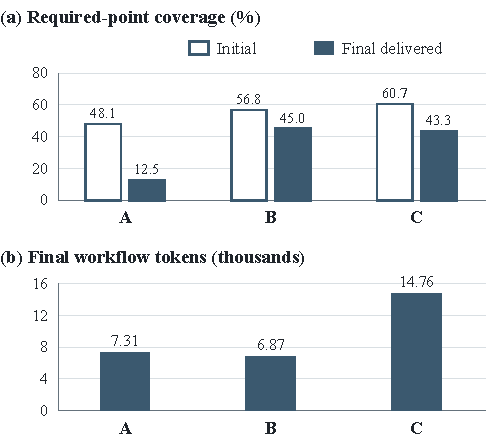
\includegraphics[width=\linewidth]{figures/coverage_cost.pdf}
\caption{The 20-case coverage--cost tradeoff. Top: initial and final delivered point coverage. Bottom: total model tokens per workflow, including evaluation but excluding shared planning and offline grading. Stages use different accounting scopes, so token bars show only the final workflow.}
\label{fig:tradeoff}
\end{figure}

\subsection{Retrieval Quality and Maintenance Cost}
Struct offers coherent evidence with fewer vectors, at the cost of coarser matches, more tokens per passage, and truncation risk. Adapted Dense shifts work offline: changing encoder weights requires training and re-encoding the corpus. Frozen retrievers with an off-the-shelf reranker avoid task-specific training but add candidate-pair scoring on every query. In principle, either a frozen adapted or untuned encoder can encode new documents without retraining; an incremental-update workflow was not evaluated. Total training, rebuilding, and maintenance costs were not systematically compared, so query latency is not a deployment-cost comparison. These BGE results do not establish downstream gains for the separate MiniLM backend.

\subsection{Routing Helps Before More Agents Help}
The matched initial B/C retrieval results suggest that the main gain comes from allocating context across domains, rather than from generating more intermediate answers. Independent generation can help locally: in case 017, the synthesized answer includes the bank-account detail missing from the pooled answer. This is useful evidence that decomposition can recover an omitted requirement, but three improved initial cases and higher aggregate cost do not justify unconditional decomposition. A sensible next experiment would trigger independent generation only after identifying uncovered subrequests.

\subsection{Approval Can Miss a Conditional Error}
Case 018 asks about identification information for FAFSA and correcting a Social Security record. B states that a driver's-license number is needed \emph{if you are not a U.S. citizen}. The annotated source condition for the license number is instead having a license; the citizenship condition belongs to neighboring registration information. The retrieved character window concatenates these neighboring items. The answer receives an online pass despite the condition mismatch.

This case illustrates why valid citations and high evaluator scores are weak substitutes for claim-level checking. A generator can use words present in a cited passage while attaching the wrong qualification to a field. Preserving list and heading structure, checking each condition against its local source span, and independently annotating claims are more targeted responses than simply increasing retrieval depth.

\subsection{Stopping Can Remove Useful Partial Answers}
The reduction from initial to delivered coverage in Figure~\ref{fig:tradeoff} is largely a release-policy effect. Once the evaluator rejects an answer, a bounded controller may correctly avoid delivering the draft, yet a generic handoff message conveys none of its supported content. Reporting coverage alongside acceptance makes this tradeoff visible. A future partial-answer policy could return independently supported portions, identify unresolved items, and request clarification or handoff for the remainder. That policy would need claim-level validation; the present logs do not establish its safety or effectiveness.

Case 009 shows an additional composition failure: C's SSA subworkflow returns an insufficient-evidence status with citations and fails validation. The final response is escalated rather than assigned an overall component-error status. A single defective domain workflow can therefore reduce the utility of a multi-stage answer even when other components return useful evidence.

\subsection{The Judge Introduces Measurement Noise}
Automatic point grading is not independent of generation. Identical B answer text in cases 005, 014, and 018 receives different point labels across the two saved batches. Thus, some apparent coverage changes reflect regrading rather than changed answer content. The paired bootstrap intervals condition on these recorded labels and cannot remove that uncertainty.

Before claiming reduced hallucination or reliable completion, we would freeze a human-reviewed rubric, obtain independent claim-level judgments, and calibrate evaluator thresholds on separate development examples. We would then run Dense-only, hybrid single-pass, evaluator-only, and full-loop configurations on the same held-out dialogue cohort. The current 1,000-request and 20-request studies use different samples and metrics, so they do not constitute that complete ablation.
